\chapter{Background}
\label{ch:background}
With the goals and objectives of the project clearly laid out, it is now necessary to explore the factors which drive digital dependence. This chapter explores the concepts in biology and neuroscience which cause "hooked" users to become unfocused and unproductive despite their best efforts to do otherwise. It will then highlight a few clear examples of how the design of modern apps leverage these concepts and then do a short review of the existing product.

\section{Biology Primer}
To develop an app to fix the problem of attention deficiency, a short exploration into the mechanics of attention preservation is necessary.
Within this scope, our focus will be on two different parts of the brain: the limbic system and the prefrontal cortex.

\subsection{The Limbic System}
The Limbic System carries out many functions that are considered "primal urges". Emotional responses to food, smell, social cognition, emotional memory and sexual behaviour \cite{rajmohan2007limbic}. All these functions can be summarised and grouped by one common concern: self and species preservation.

The limbic system (henceforth referred to as the "chimp"), is adept at remembering emotional responses to previously experienced situations and inducing the optimal response for self-preservation, should it find itself in a similar one. These responses can be associated with negative emotions, such as the fear one experiences when spotting a predator, or positive, such as the satisfaction and drive upon finding a food source. This is a gross over-simplification of the capabilities of the limbic system, but the message is clear: it is the part of the brain responsible for learning and inducing impulses that it deems will result in the highest chances of evolutionary survival and comfort.

However, with respect to self-control and achieving one's long term goals, this may be undesirable. The stress hormone (cortisol) produced when working under tight deadlines with complex problems is not unlike that produced in life-or-death situations in the wild. The chimp has no way of differentiating this and therefore the stress response induced by work is biologically registered as an existential threat, which encourages impulses of procrastination or indulging in escapism as part of a "fight-or-flight" response.

\subsection{The Prefrontal Cortex}
The Prefrontal Cortex (PFC) is the part of the brain largely associated with conscious thought and rational self-control. An extremely well-cited study by Miller and Cohen \cite{miller2001integrative} concluded that in general, actions that require critical thought against our base instincts always involve the engagement of the PFC, and that test subjects with PFC impairment performed poorer on such tasks. One such example was the sorting of cards by the colour verbally printed on them, even when the card itself was another colour (e.g. a blue card with the word "red" printed on it would be classified as red).

One prevailing theory is therefore that the PFC and the limbic system are often at odds in tasks involving self-regulation \cite{heatherton2011cognitive} and that successful self-control is a balancing equation of the strength of so-called "bottom-up" impulses and "top-down" conscious thought. This sets the stage for our narrative: that the "chimp" within us and the "human" are always at odds when it comes to work and procrastination. While the PFC may wish to act in favour of our long-term goals, it often loses to the "chimp" and we are left with only a running commentary on our actions, despite our best wishes to do otherwise.

\section{Self-regulatory Failure}
Resisting the urge to check one's phone or play video games is a prime modern example of self-regulatory failure that reflects much in common with addiction-like behaviour in dieters, smokers and substance abusers. App-fueled procrastination may not be as lethal as substance abuse or obesity, but there nonetheless exists a very slippery slope into internet addiction that may ensnare the average person. Heatherton and Wagner elaborate in \cite{heatherton2011cognitive} that there are a few common causes for self-regulatory failure, which can be separated into two categories. "Top-down" factors are associated with reduced capacity or strength of conscious self-control such as negative moods and self-regulatory resource depletion. "Bottom-up" methods refer to unconscious or natural impulses such as cue exposure or lapse-activated consumption.

\subsection{Resource Depletion \& the Strength Model of Self-Control}
Baumeister and Heatherton \cite{baumeister1996self} initially proposed in 1996 that conscious self-control against one's impulses draws from a global resource pool that depletes as one uses it further. Since then, many studies have released results in support of this hypothesis. The strength model dictates by construction that it is possible to exhaust one's self-control and must be replenished like any other resource.

This suggests that as long as a distracting alternate stimulus is present, self-regulatory failure is not a question of "if", but "when". For traditional office work settings, this effect is ameliorated by the social norms enforced by the office culture. However, for a person working from home, the distraction unfortunately exists on the same device that enables productivity and there are no sources of social pressure in play to keep the chimp in check.

\subsection{Cue Exposure}
A cue in this context is defined as a piece of sensory stimulus which has an association to a certain consumption-related behaviour. Take for example he smell of food for a dieter or the sight of a beer for a heavy drinker. Cues have been shown to increase cravings, draw attention and increase likelihood of consumption \cite{jansen1998learning}. Furthermore, multiple studies \cite{stacy2010implicit} have shown that individuals are often unaware of how cues affect them on a conscious level, and so it becomes difficult for a struggling individual to pinpoint what it is exactly that causes their self-control to lapse.

The first example of addictive software engineering is the push-notification, one of the core tools of user-experience (UX) design. The premise seems simple: software engineers needed a way of bringing a user's attention to key information. This is not a "new" phenomenon, as pagers and message alerts have been around for as long as phones have existed. However, the capabilities of the smartphone take these alerts to a new level. The modern push notification engages many senses: a kinetic vibration (which is audible even if the phone is silent!), an audio alert and a visual alert window.

Both Android and iOS have robust application programming interfaces (APIs) that enable developers to exercise a very high level of control over how their app sends and handles notifications \cite{androidnotification}. In the example of a social media message from a friend, this allows for extremely alluring design: an avatar of the friend and a short preview of the incoming message. Users are even empowered to make the experience of receiving a notification as enjoyable for themselves as possible. Facebook Messenger allows users to set nicknames for their friends. Most phones allow users to set specific alert sounds on a per-contact basis, allowing a user to know from audio perception alone who they are receiving a message from. While this feature feels like one that helps the user "filter out the noise", one might argue that it in fact facilitates distraction, by allowing the user to have a stronger, more focused response to a self-set cue.

Cue exposure need not even be as explicit as a push notification. The experience of using a social media app or playing a game is extremely pleasurable. Beautiful colour palettes, high-resolution artwork and buttery-smooth animations are a staple in successful apps. All these factors enable the "chimp" to register a positive emotional response to act of phone use in what we call an "internal trigger" (more on this later). Therefore, the very presence of the phone is a form of cue exposure that constantly forces the user to exercise self-restraint.

\subsection{Lapse-activated Consumption}
A 1975 study \cite{herman1975restrained} showed that the consumption of a small amount of an addictive substance (in this case, a milkshake on a test audience of dieters) paradoxically caused dieters to consume more food afterwards, in contrast to the control group of non-dieters who ate less. Similarly, many of us find that picking up our phones for a short break or otherwise directed task can often snowball into a longer-than-intended session which comprised of all manner of actions unrelated to why we originally picked up the phone. Playing "just one round" of a video game often ends up being anything but.

Apps offer extremely dense experiences that engage visual, auditory and even kinesthetic senses that are highly appealing to our physiologies. Levy and colleagues \cite{levy2016effect} showed that not only is the occurence of a disturbance a problem, but the "richness" of that disturbance was also detrimental to subjects' performance on cognitive tasks. This explains the unconscious effect that distraction has, and why people find it difficult to go back to work once they have been distracted by a form of smartphone media.

The exact reason as to why lapse-activated consumption occurs is not fully clear even with current research, but the implications of its existence are. Humans are unfortunately pre-disposed to "falling off the wagon" once an attractive enough stimulus is presented. We will soon explore how smartly designed apps leverage this as an entry point to their user experience and place the user into a continuous loop of habit-forming app use.

\section{Motivation and Persistence}
We have seen so far that the outcome of a self-restraint task comes down to whether the strength of bottom-up impulses exceeds that of our top-down intentions. Most of the time, this tends to be the case. Having explored all the ways in which self-control can fail due to how strong our in-built tendencies are, perhaps then there is a way in which we may use these natural tendencies to our advantage, or at least increase the strength of top-down control.

\subsection{Strengthening Self-control}
% How can one increase their desire and motivation to work on long-term goals?
Muraven, Baumeister and colleagues \cite{muraven1999longitudinal} conducted a study in which subjects performed consistent amounts of self-enforced exercise over two weeks. While this caused slightly decreased self-control capability for a short refractory period after, this ``strength drain" diminished rapidly by the day and eventually resulted in increased success in other completely unrelated self-restraint tasks. Muraven \cite{muraven2010practicing} took these results again in a later study and found that "smokers who squeezed a handgrip or avoided sweets for two weeks before quitting cigarettes remained abstinent longer and had fewer lapses overall as compared to smokers who practiced tasks that did not require self-control".

% Is there any way to convince the chimp to want to do work?
These studies, and many others like it, strongly support the previously mentioned strength model of self-control. Metaphorically, self-control behaves very much like a muscle: its capabilities are slightly diminished following immediate use and while it is possible to fatigue it significantly, it is also possible to increase its capabilities with consistent amounts of progressive load.

\subsection{Impairing Impulses}
Cinciripini and colleagues \cite{cinciripini1995effects} investigated the effects of schedules and gradual consumption reduction in smoking cessation. Participants were all given uniform education on the physiology of nicotine addiction and methods of coping. Control over consumption was exercised in two forms: scheduling, where participants were allowed to smoke at designated and progressively lengthened intervals, and reduction, where consumption was reduced by a third of the subject's baseline consumption each week. The scheduled and reduced group unsurprisingly performed best, with the greatest reduction in mean cigarette consumption and reduced frequency of urges and severity of withdrawal symptoms. Reduction alone contributed most to the reduction of urge frequency, and scheduling seemed to have an effect on mean consumption.

Results from studies such as these suggest that the controlled appeasement of urges may be a key factor in helping to diminish the effects of bottom-up impulses and serve as a basis for productivity schedules such as the pomodoro technique, which is based on using 25-minute focused intervals of work with short breaks in-between to maximise the extent of a given individual's attention and focus.

\section{Addictive Design}
The principles of behavioural science examined so far dictate that a successful well-being app has to not only help the user form healthy habits that help them avoid self-regulation pitfalls, but also offer new "hooks" to help to keep their inner chimp from becoming overly restless. As a first step in this endeavour, we shall study in this section a few detailed (but not exhaustive) examples of how apps create an addictive experience for their users.

\begin{figure}[h]
    \begin{center}
        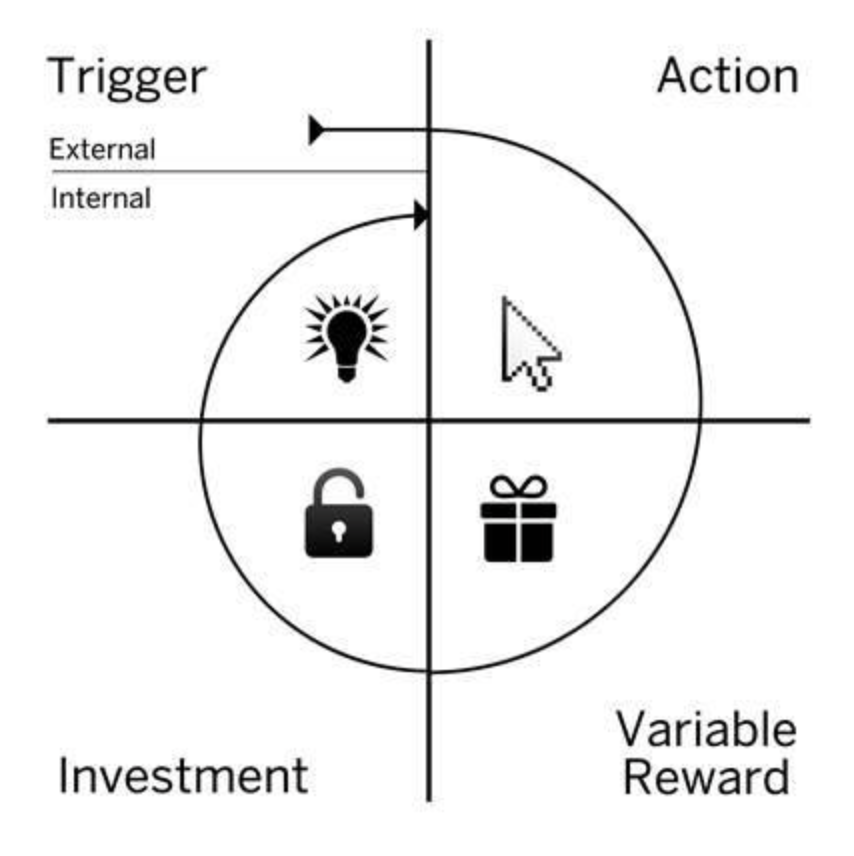
\includegraphics[scale=0.3]{images/hook_model.png}
    \end{center}
    \caption{The 4-stage Hook Model.}
    \label{hook_model}
\end{figure}

This project uses the concepts laid out by Nir Eyal \cite{eyal2014hooked} in his book about habit-forming software design, "Hooked". He lays out the hook model, which consists of 4 phases: Trigger, Action, Variable reward and Investment.

\subsection{Trigger}
Bearing the exact same meaning as it does in the case of substance addicts, the trigger is any form of cue exposure that is deliberately aimed at getting the user to perform a desired behaviour. In the world of user interaction studies, we call this a "call-to-action".  Eyal broadly separates these into two categories: external and internal triggers.

Anyone who owns a smartphone immediately relates to the concept of an external trigger. A push notification, message, email, or toast-style pop-up within an app all are perfect examples. They bring to our attention a piece of often enticing information, causing us to react. In fact, in the process of trying to make a minimum working example for this project, the wonderful engineers at Google have sent us a perfect example of an external trigger, shown in Figure \ref{fig:firebase_cue}.

\begin{figure}[h]
    \begin{center}
        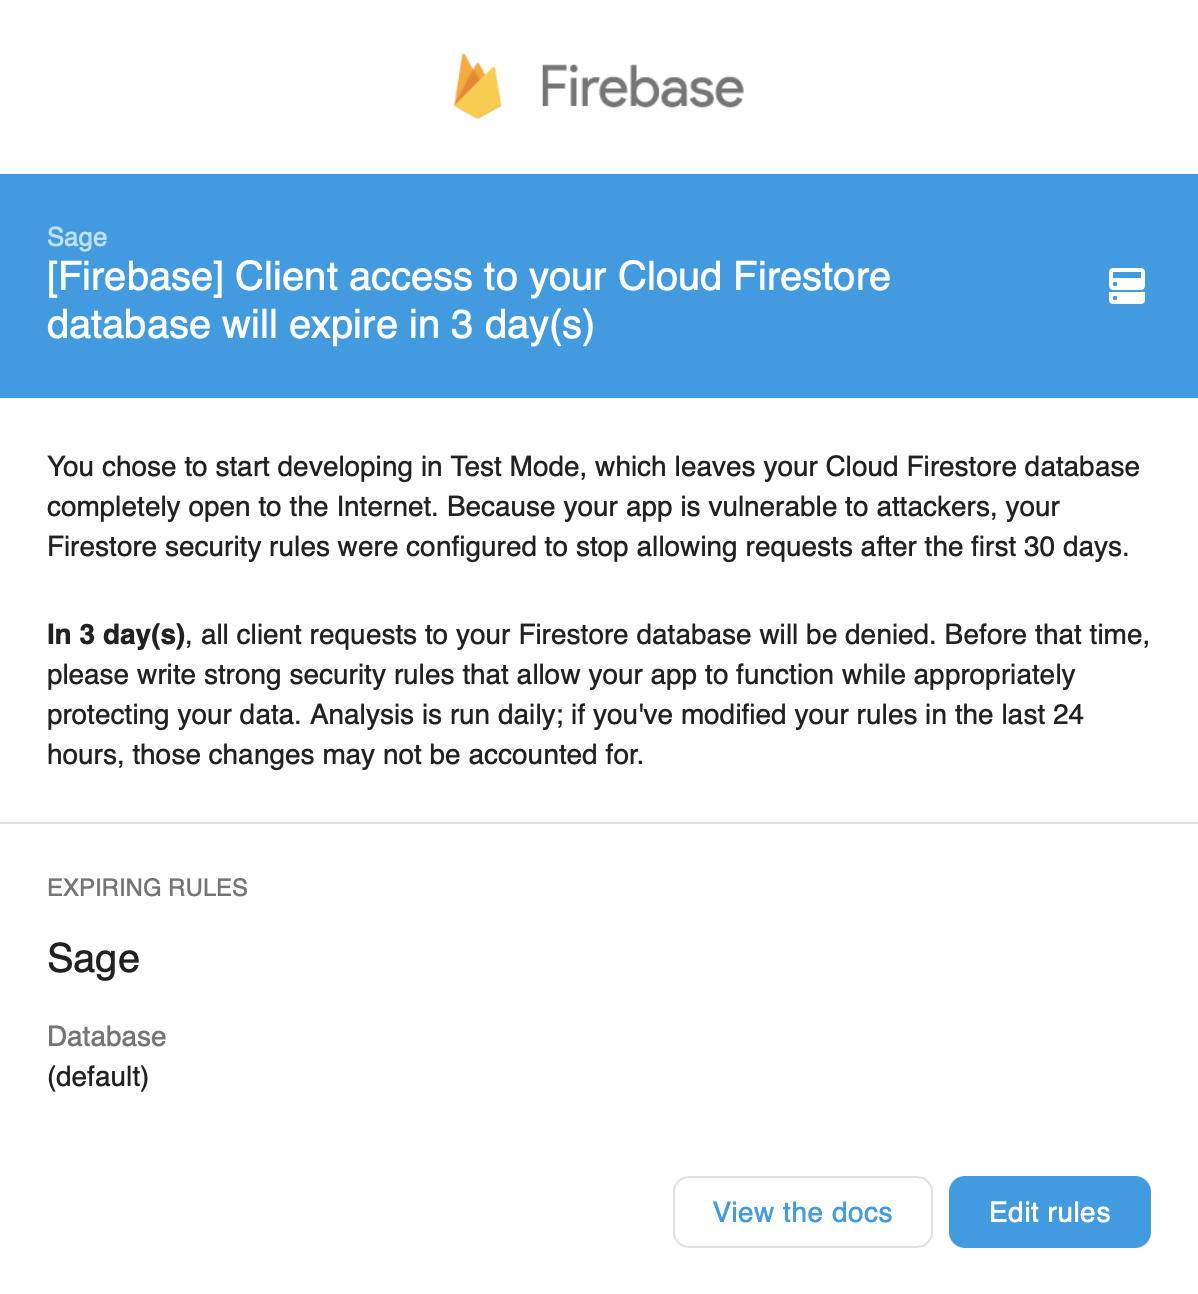
\includegraphics[scale=0.3]{images/firebase_cue.png}
    \end{center}
    \caption{An external trigger from this very project's cloud service provider.}
    \label{fig:firebase_cue}
\end{figure}

The logo at the top immediately reminds us of who we are receiving this email from. A calming light blue panel greets us in the middle of a surrounding of off-white, providing high contrast and yet being easy on the eyes. The message is extremely clear, highlighted within the accessible, high-contrast colour panel and enlarged font.  The detail text in the middle satisfies the more discerning individual, but is almost completely unnecessary, as the panel below it tells the entire story in a beautifully minimalistic fashion. It tells us \textit{exactly} what is happening, to which database, and even provides clearly described high-contrast elements that are clearly interactable, allowing us to take action immediately. Each element in this panel is given its own generous amount of real-estate on the screen, helping the user to hone their focus and drawing attention to the correct elements.

This email is directed at someone deep in the user journey, not even at "hooking" a new user into the platform. Even then, the amount of attention to detail and incredible design cannot be overstated and the trigger achieves its goal perfectly. Through careful planning, Firebase has successfully anticipated the exact courses of action that a developer might want to take with regard to this piece of information, and has made it as painless as possible for the user to actuate it.

Internal triggers are much more subtle, and are the result of an emotional coupling (remember the limbic system!) of a specific thought or feeling with the product. One can argue that the reason for the massive success of addictive apps is that, similar to drugs, they provide a euphoric escape to the otherwise negative emotions that their users face on a daily basis. Childress and colleagues \cite{childress1994can} found that hypnotically-induced negative moods such as anxiety and depression produced significant increases in self-rated cravings in detoxified opiate abuse patients. Similarly, loneliness, anxiety, boredom and depression can be temporarily escaped with the hit of dopamine that the app experience provides (more on this in the section on variable rewards). This conditions an internal trigger in the user: "When I am sad or lonely, talking to friends on Facebook makes me feel less so".

This is the power of the trigger. It is the first step in a continuing feedback loop which motivates or otherwise plant an intent within the user. Triggers may be coordinated and put in place all over the user journey for a variety of different outcomes.

\subsection{Action}
Fogg's behaviour model \cite{fogg2009behavior} summarises the mechanisms of user action elegantly: "Behavior (B) happens when Motivation (M), Ability (A), and a Trigger (T) come together at the same moment". To increase the odds of a user performing an action we desire, all three elements must be present, and in sufficient quantity to cross a so-called "decision threshold".

\begin{figure}[h]
    \begin{center}
        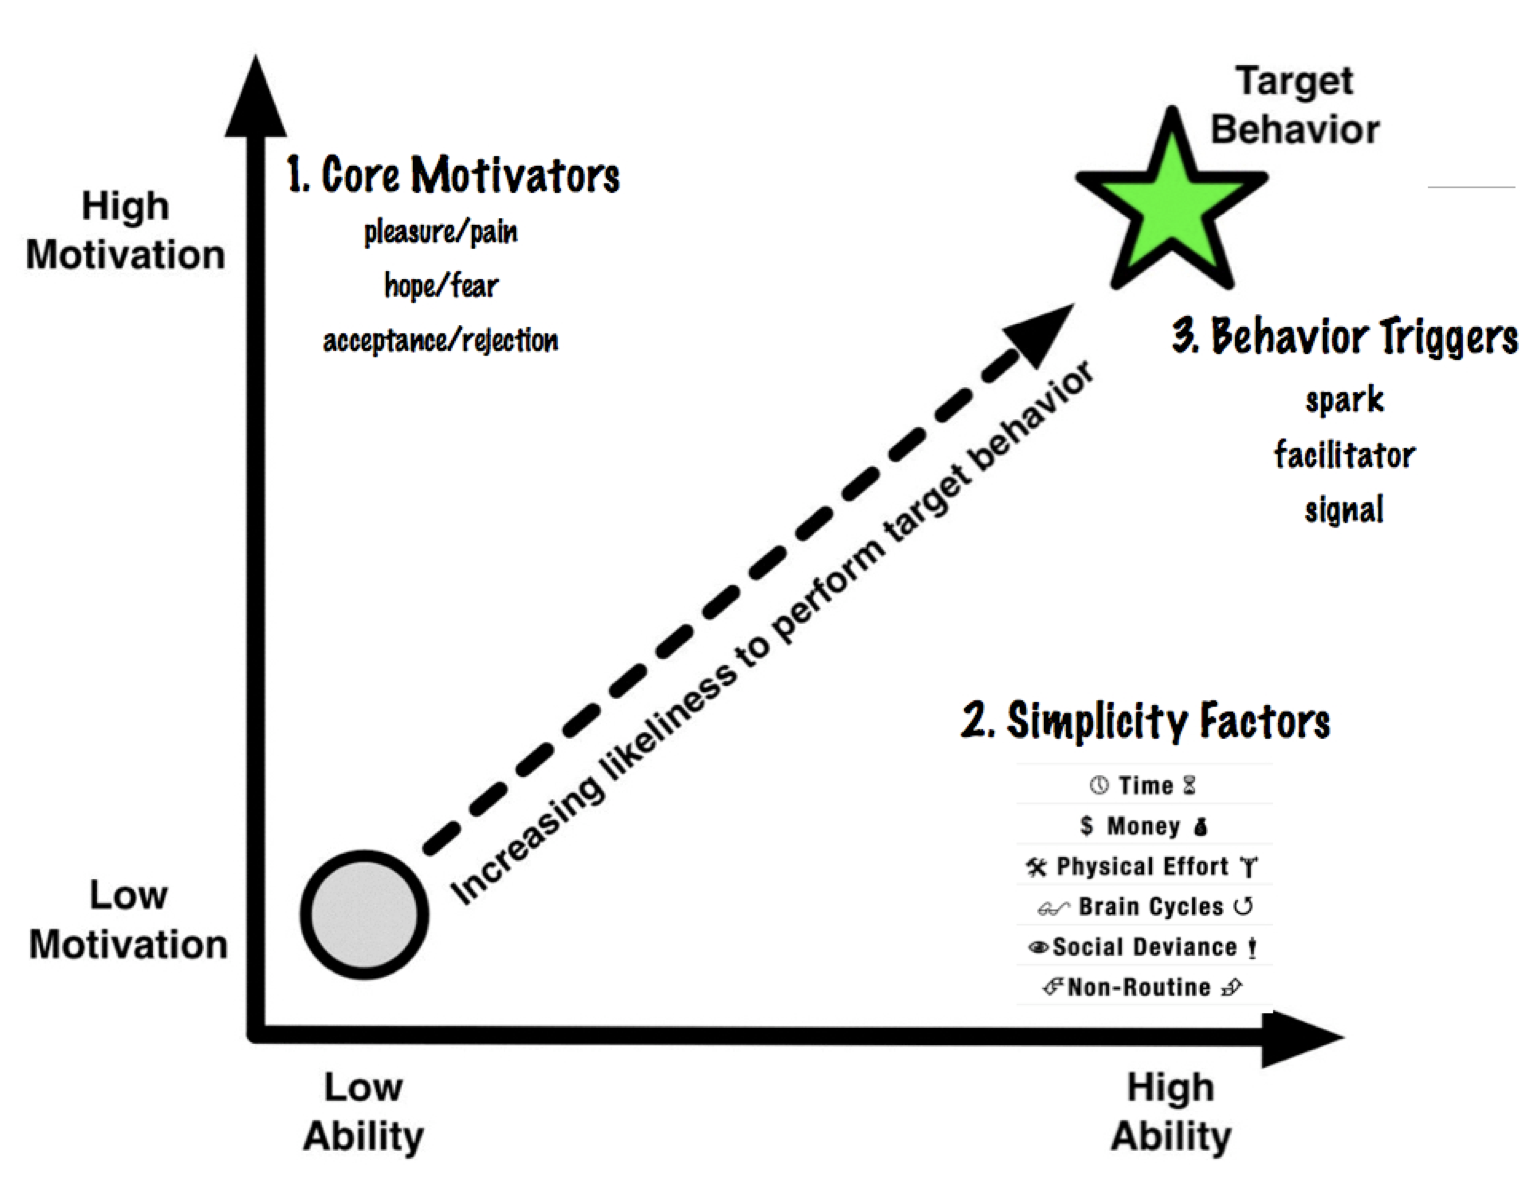
\includegraphics[scale=0.3]{images/fogg_behaviour.png}
    \end{center}
    \caption{The Fogg Behaviour Model as illustrated in the original paper.}
    \label{fig:fogg_behaviour}
\end{figure}

Having already covered triggers and how they may be used to spark motivation, this section mainly discusses ability. The example in the previous section is an excellent example of how interactive elements can be carefully placed to make action as easy as possible for the user. This highlights the fact that motivation and ability can trade off, as a highly motivated user may be willing to go through more work in order to achieve a desired outcome. Ease of use is much more within developers' control than user motivations and intentions. If a developer can design the interaction such that all the "simplicity factors" expended (in figure \ref{hook_model}) are minimised on behalf of the user, the product feels intuitive and users can simply act on instinct rather than constantly deplete precious reserves of cognitive effort.

A quick moment of reflection will reveal that many of the features that we consider to be excellent are the ones that do precisely this. The widely adopted "Sign up with Facebook" feature completely removes the barrier of entry that new users usually have to go through to access a site. Most modern smartphones have access to their cameras without requiring an explicit unlock. E-commerce retailers often allow users to subscribe to email updates to know when a specific product is back in stock. The list goes on and is endless, but it is clear that usability is a key factor in app design, allowing users to spend increased amounts of time in a given app without feeling the strain of prolonged cognitive effort or other resources.

\subsection{Variable Reward}
We have known since the times of Pavlovian conditioning that rewards condition a learned response in animals. Science has since then come a long way in helping us understand the mechanisms responsible for motivated action in humans and animals. The neurotransmitter responsible in many of these motivating behaviours is Dopamine. Dopamine travels through various parts of the brain through well-known pathways, and each of these pathways is responsible for feelings of pleasure and reward such as during sexual intercourse and eating food (particularly foods high in sugar).

However, dopamine is not only released upon the actual experience of a positive experience, but in anticipation of one. A study by Salimpoor and colleagues \cite{salimpoor2011anatomically} conducted a study on dopamine release and music. It showed that contrary to belief at the time, dopamine was released distinctly in different pathways at two moments: in anticipation of a moment of peak emotional arousal, and during the actual moment itself. One of Schultz's \cite{schultz2016dopamine} many extensive works on dopamine-reward mechanics also builds upon long-standing models in neuroscience which state that the brain uses dopamine to learn emotional responses by comparing the anticipatory and actual response upon receiving the reward. Schultz showed that the dopamine neurons showed the greatest activity when the received reward exceeded what was anticipated, therefore resulting in the greatest learned behaviour. If a reward was anticipated but an underwhelming (or negative) result was actually received, the latter dopamine response is practically nonexistent and the brain associates this to a negative experience.

Variable rewards in apps exploit this in one of two ways: either providing a reward when one was not expected, or by having a low-calibrated expected reward and providing a much larger one (eventually). The addictiveness of this variability has been shown to be extreme. The classic experiment conducted on mice by Olds and Milner \cite{olds1954positive} connected electrodes directly to the pleasure center in test mice and placed them in a chamber where they could press a button to stimulate themselves. When the reward was made variable (given after a random number of button presses), mice lost interest not only in food and drink, but even sexual reproduction. A later study \cite{berns2001predictability} confirmed with fMRI scans that humans had higher brain stimulation levels when the potential reward was variable, and not predictable.

Taking this knowledge in the context of primitive human biology, Eyal \cite{eyal2014hooked} describes that rewards fall into three general categories: the tribe, the hunt and the self. Simply put, humans crave rewards from social acceptance, reward-for-effort and self-accomplishment and improvement, respectively. One does not have to be a genius to see how these exist in the design of social media apps. Facebook and Instagram give users social acceptance in the form of statistics on their content, such as the number of "likes" from friends, and even have social interaction built in to features such as comments and in-app messengers. Such updates happen completely randomly from the perspective of the user, as they are actuated by other users. It is therefore very common for social media app users to feverishly open the app, even when no explicit notification has been received. Even if no direct response from a friend was expected, apps still employ machine learning algorithms to place a tailored content feed in front of the user when they open the app, providing a reward even when none was expected. Over time, this results in a conditioned response of opening the app in expectation of some unknown abstract reward, and an internal trigger is formed that tethers the mere opening of the app to a positive, rewarding experience.

\subsection{Investment}
The final phase of the 4-step hook model requires the user to perform an investment in the product. This is not necessarily monetary, but rather refers to the user placing some form of effort into the system. This is slightly contrary to the principles of action mentioned before, in which effort on behalf of the user was minimised. In order to get users to willingly put in this investment, it is usually prompted after the user has received a variable reward. This, according to Eyal \cite{eyal2014hooked}, plays on the human tendency to reciprocate to kindness. Other motivating factors for a user to contribute may be similarly built up by the app. Humans enjoy consistency with past behaviours and dislike cognitive dissonance, where one's actions may be in conflict with one's beliefs. We will see in the following example how these can be exploited.

Investment can come in many forms, and often apps find a way to make users feel a sense of ownership over their investment, even if it offered no direct benefit to them. Many of the most successful apps have some form of recommender system within them. Google Maps, for example, is essentially a large geographical recommender for a user's desires. Apart from its explicit use as a navigation tool, it allows the semantic search of locations, such as when one types "Japanese restaurant" or "hairdresser". Clearly, Google does not deploy an army of employees to log each and every establishment in the world. Google Maps is only as good as the data it collects, which comes from its users!

For those who are unfamiliar, Google Maps offers a comprehensive navigation experience to a location of your choice. If we were to use it to get to a restaurant for a date, Google would later leave us a notification that brings us to the "contribute" screen of the app, pictured in \ref{fig:gmaps_contrib_home}.

\begin{figure}[htb!]
    \begin{center}
        \begin{subfigure}{.3\textwidth}
            \centering
            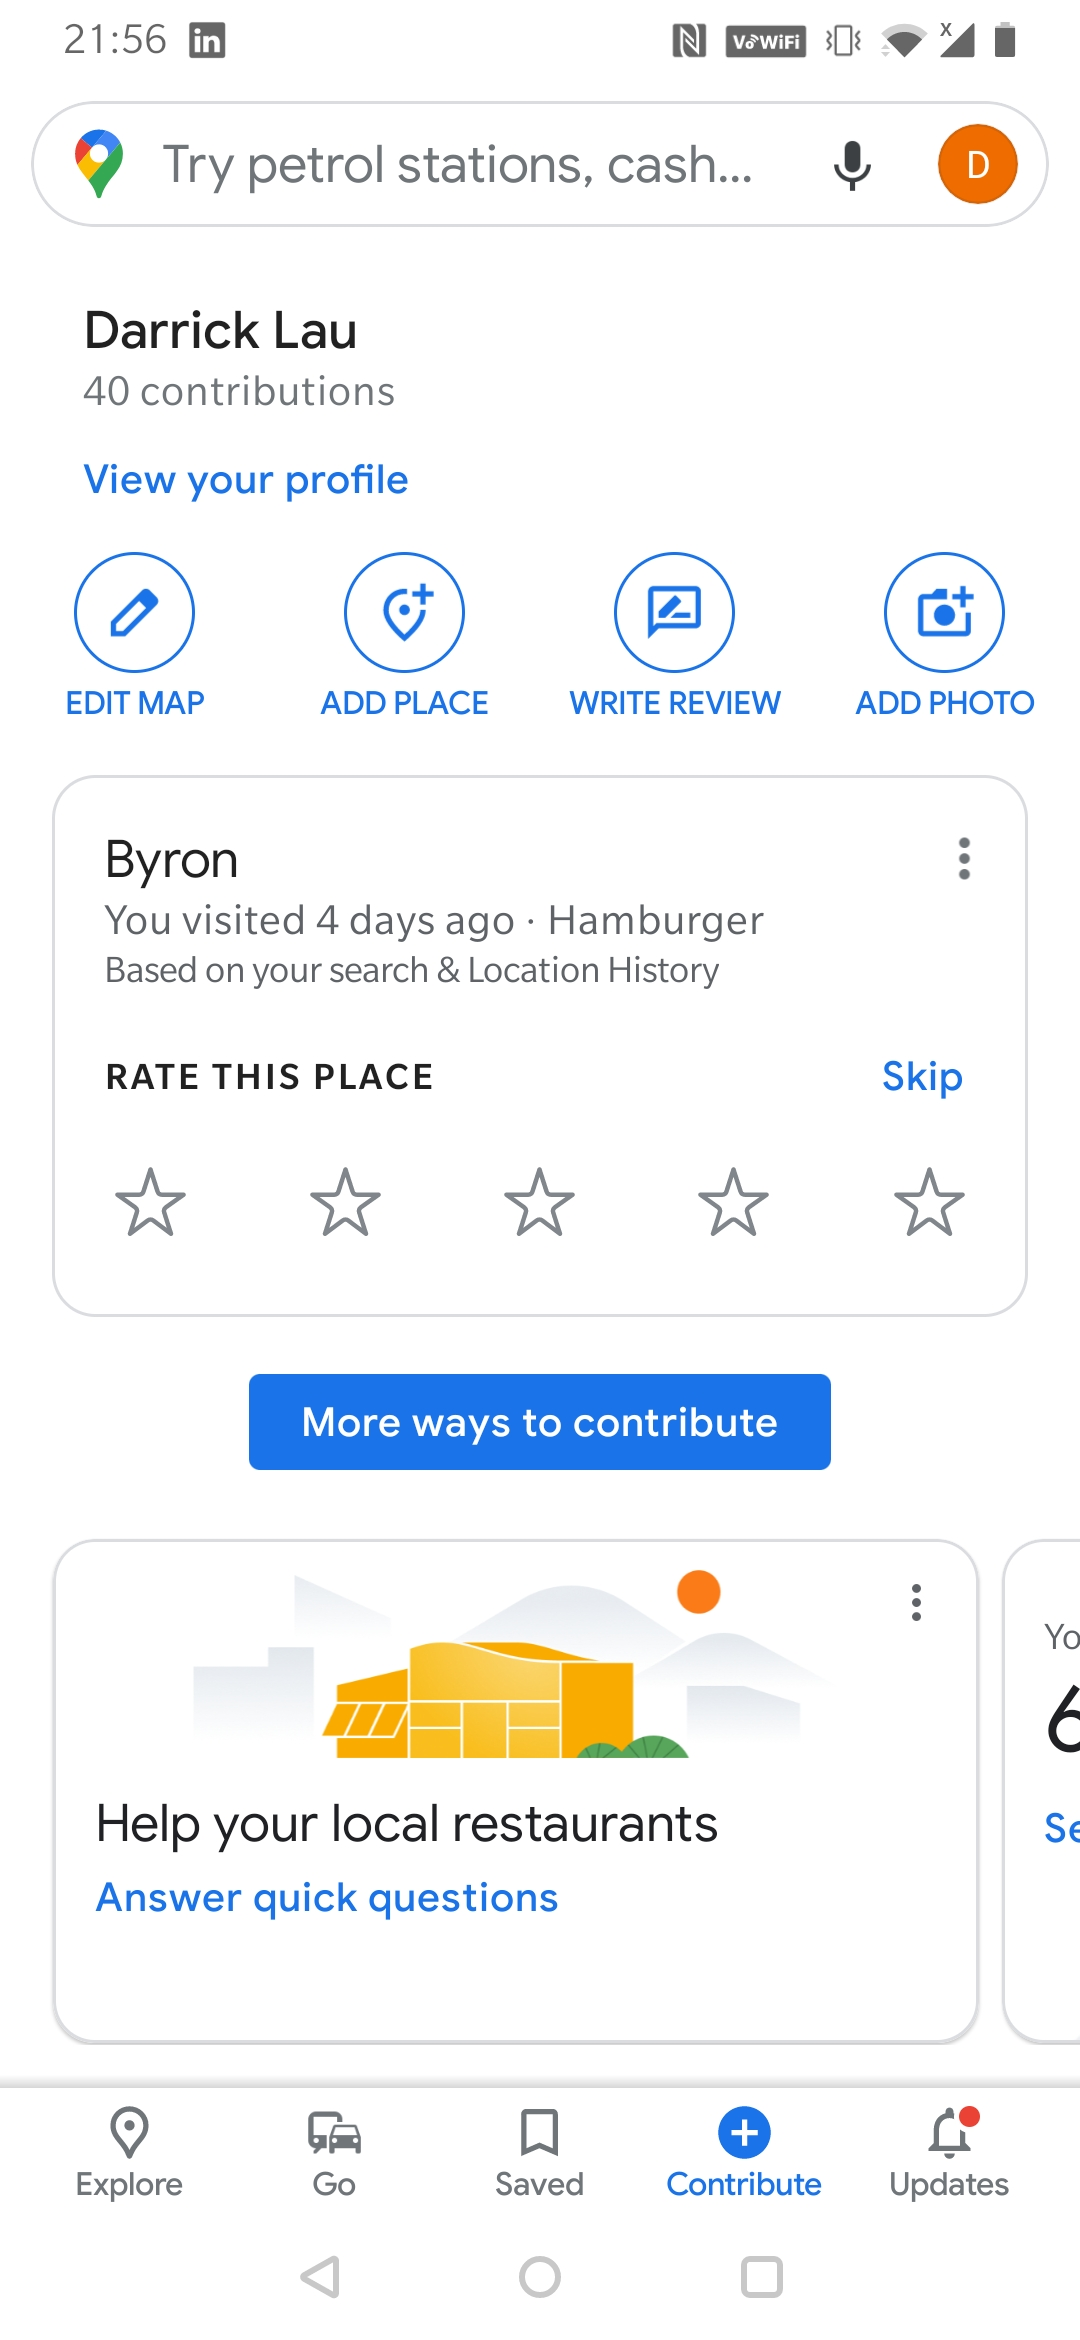
\includegraphics[width=0.8\linewidth]{images/gmaps_contribute.jpg}
            \caption{The home page.}
            \label{fig:gmaps_contrib_home}
        \end{subfigure}%
        \begin{subfigure}{.3\textwidth}
            \centering
            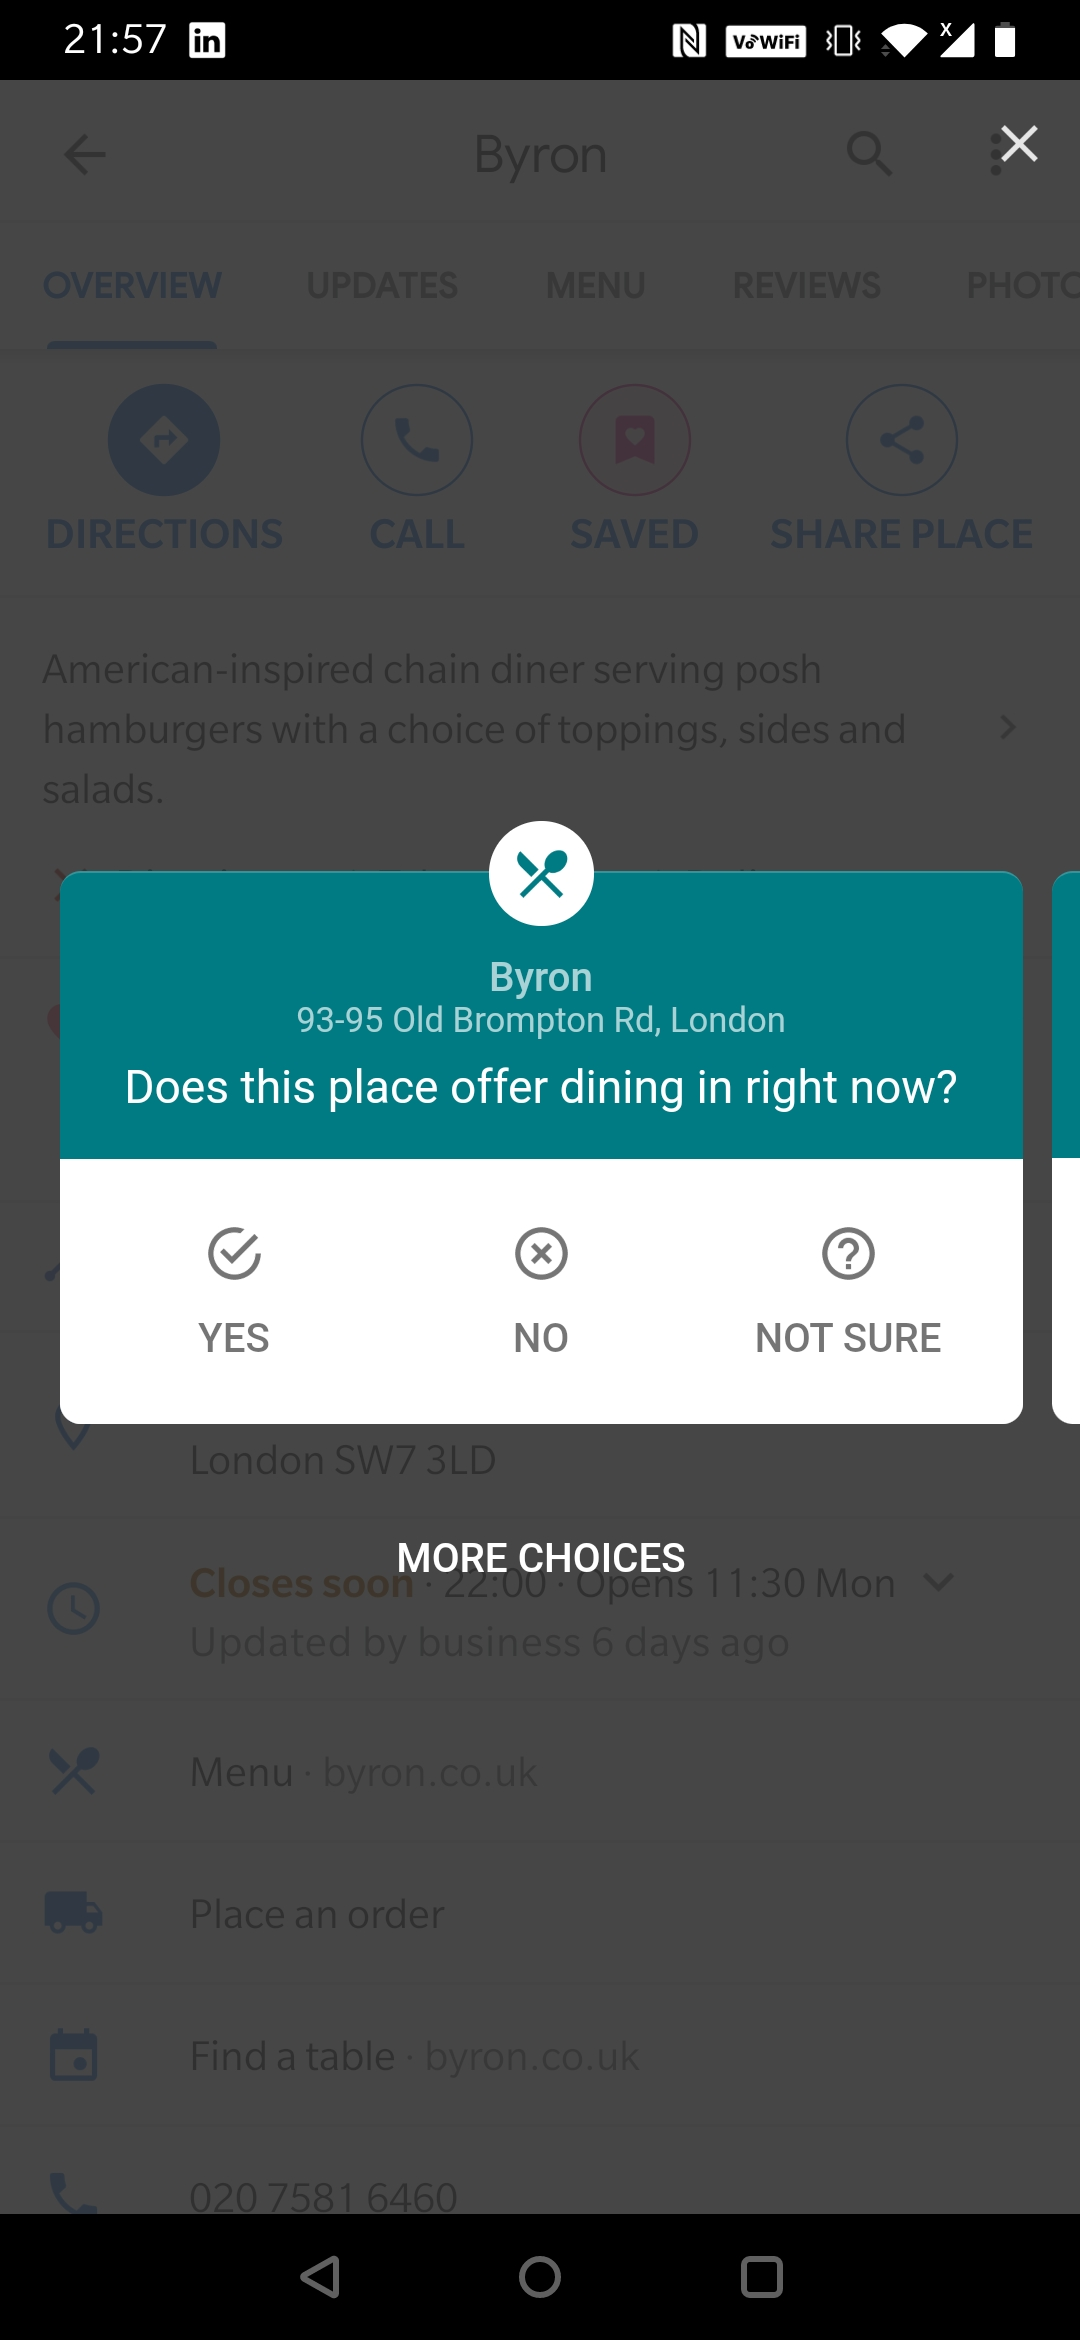
\includegraphics[width=0.8\linewidth]{images/gmaps_contribute_survey.jpg}
            \caption{A survey question about a given establishment.}
            \label{fig:gmaps_contrib_survey}
        \end{subfigure}%
        \caption{The "Contribute" Section of the Google Maps App.}
        \label{fig:gmaps_contribute}
    \end{center}
\end{figure}


This is a precise example which highlights the concepts of user investment. Having received the benefit of the wonderful navigation services Google kindly offered (for free!), the user is now given a chance to ``Help your local restaurants''. The request is made after having received some benefit, and offers the user a chance to not only reciprocate in kind to the app, but to perform an action that identifies them as a helpful member of the community (which, for most people, lines up with the image they would want to have of themselves).

The review process is exceedingly simple. Users may go out of their way to write an open-ended review with pictures of the establishment, or simply answer a set of pre-determined questions that Google has set, all not requiring open-ended answers (Figure \ref{fig:gmaps_contrib_survey}). In either case, the user is thanked with colourful confetti explosions upon completion, and the congratulatory screen is shown (Figure \ref{fig:gmaps_gamify_congrat}).

\begin{figure}[htb!]
    \begin{center}
        \begin{subfigure}{.3\textwidth}
            \centering
            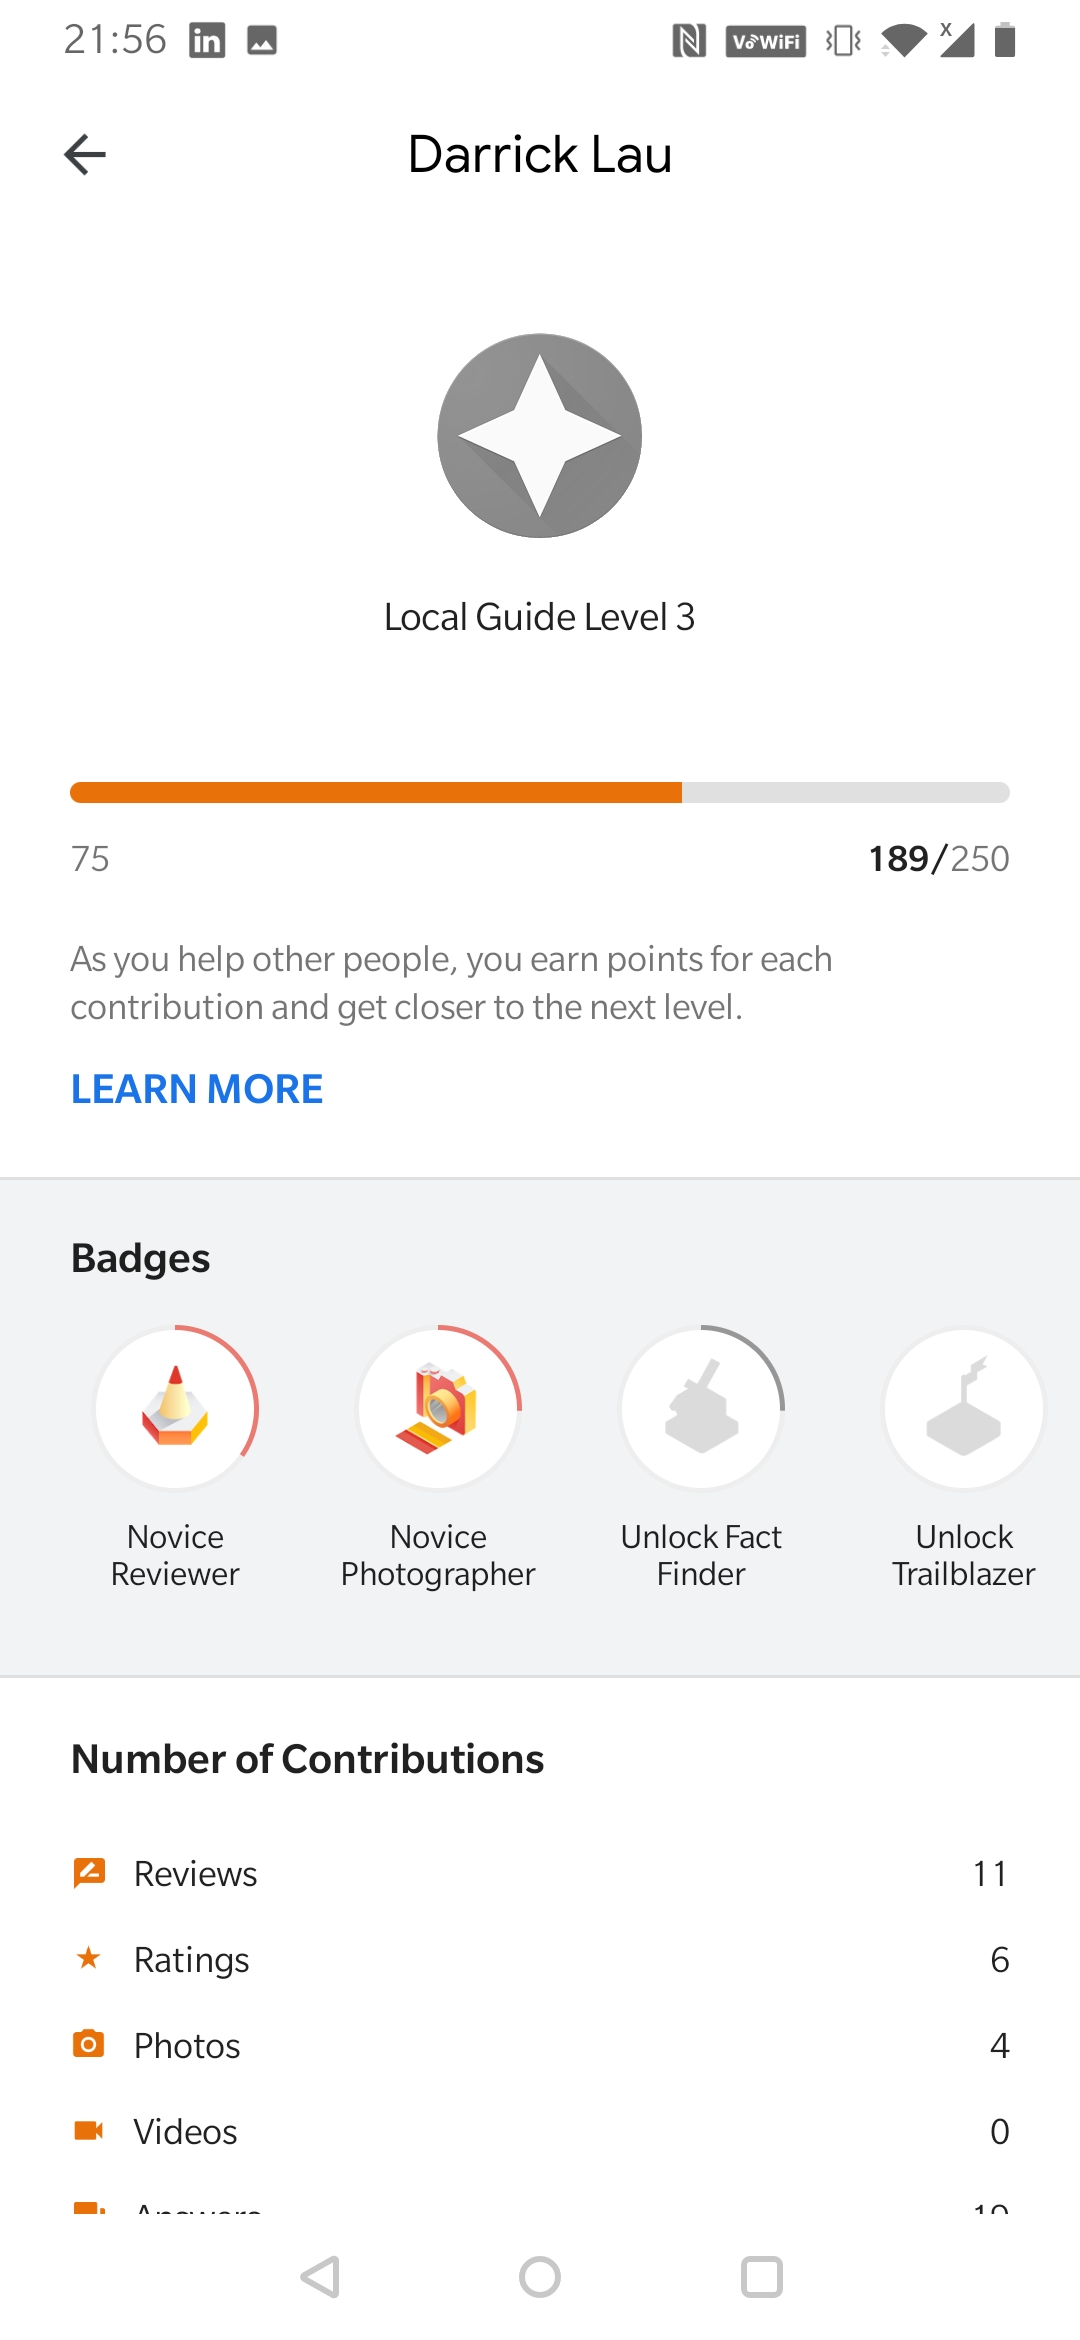
\includegraphics[width=0.8\linewidth]{images/gmaps_gamified_home.jpg}
            \caption{Google Maps contributor profile}
            \label{fig:gmaps_gamify_home}
        \end{subfigure}%
        \begin{subfigure}{.3\textwidth}
            \centering
            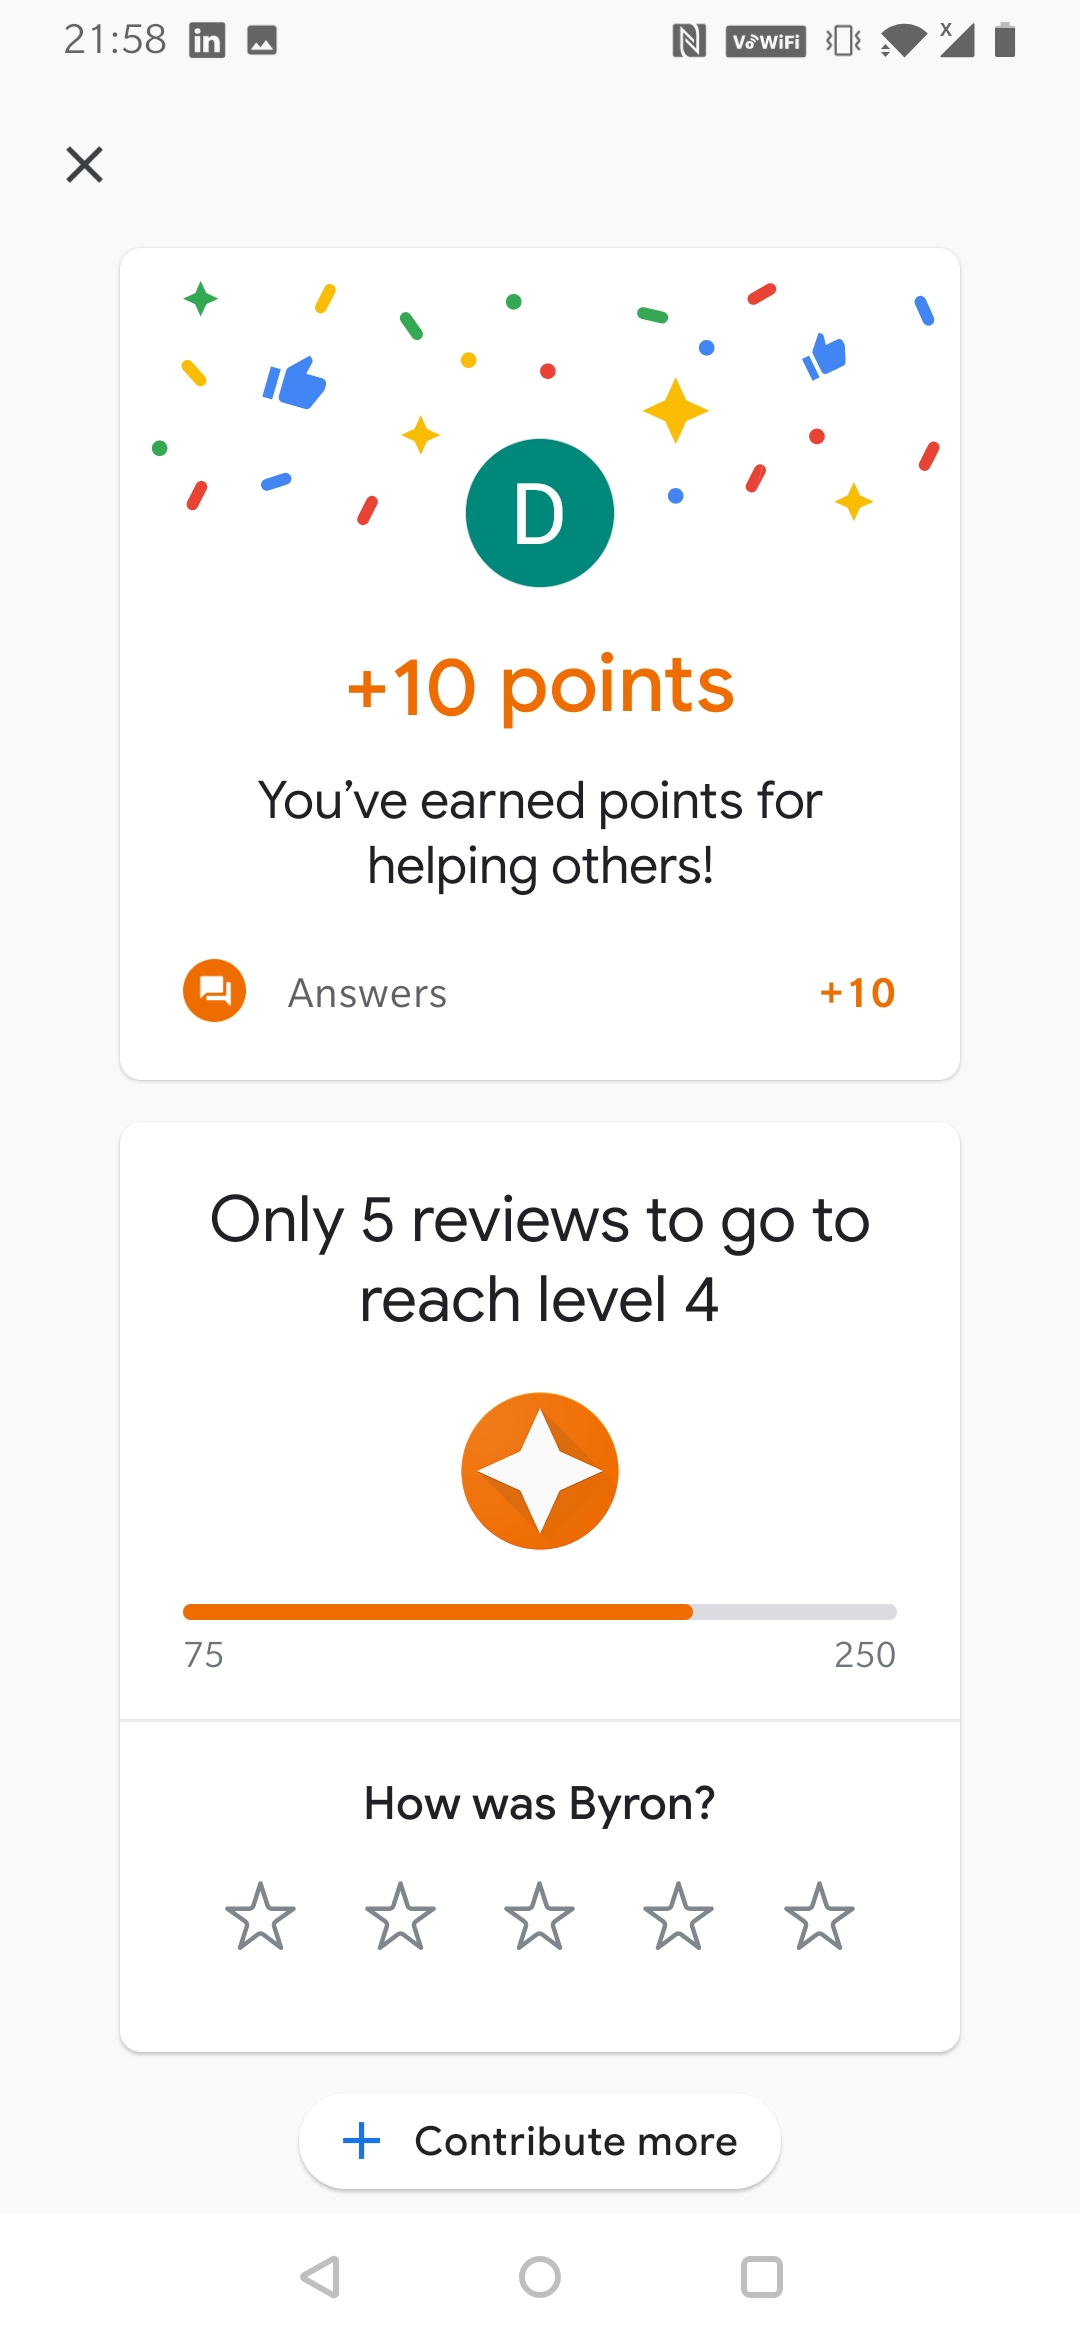
\includegraphics[width=0.8\linewidth]{images/gmaps_gamified_complete.jpg}
            \caption{A congratulatory message upon contributing.}
            \label{fig:gmaps_gamify_congrat}
        \end{subfigure}%
        \caption{The gamification of user contribution.}
        \label{fig:gmaps_gamification}
    \end{center}
\end{figure}

This brings to mind another concept: ownership and gamification. Much like classic role-playing games such as World of Warcraft, the user is bestowed a sense of ownership by building up a profile of ``achievements" by contributing to the app, and their efforts are celebrated with colourful badges and titles (Figure \ref{fig:gmaps_gamify_home}). The user is now not only increasingly attached to the product, but actively takes pride in helping to improve it on behalf of the developers.

\subsection{Concluding Statements on Addictive Design}
It is concerning that terms such as ``habit-forming products" have been thrown around so freely and only ethically questioned in the past few years. Admittedly, none of these concepts are insidious in and of themselves. One would argue that Google Maps, despite starring in these examples, has largely been an extremely beneficial product for modern society (Not many people suffer from addiction to Google Maps). However, it is clear that larger social media apps have iterated many times upon their original product and achieved a very successful application of these principles in their software design. Large amounts of money are dedicated to User Experience research in universities and internal departments in modern companies in pursuit of furthering the art of product design.

Ethics aside, one cannot expect a corporation not to take every action possible to optimise its revenues. To date, no legislation exists to govern the principles of addictive software design, and we argue that it would be very difficult to do so even if lawmakers wanted to do something about it. The best solution in the interim would be for this information to be widely available such that users at least are made conscious of how apps on their phones may be driving their unconscious behaviours.

\section{The Existing Sage Application}
Having now briefly covered the mechanics of human attention and addictive app design, a critical inspection of the current platform is necessary in order to determine the ways in which we might go about improving it.

\subsection{Functional overview}
\begin{figure}[htb!]
    \begin{center}
        \begin{subfigure}{.3\textwidth}
            \centering
            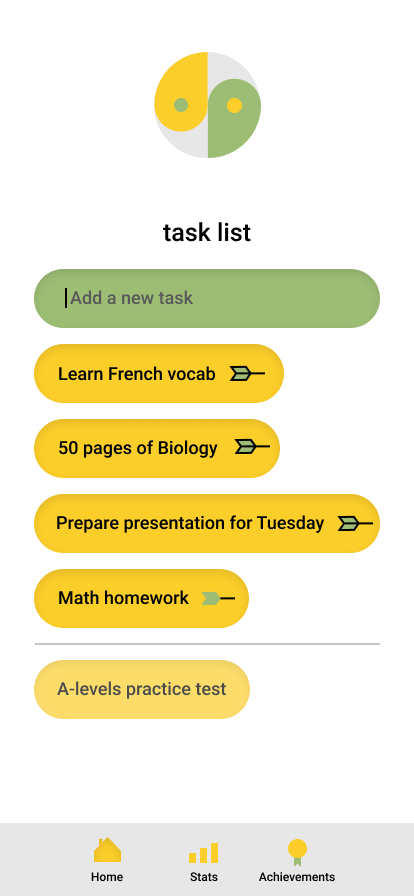
\includegraphics[width=0.8\linewidth]{images/sage_home.png}
            \caption{Home page}
            \label{fig:old_sage_home}
        \end{subfigure}%
        \begin{subfigure}{.3\textwidth}
            \centering
            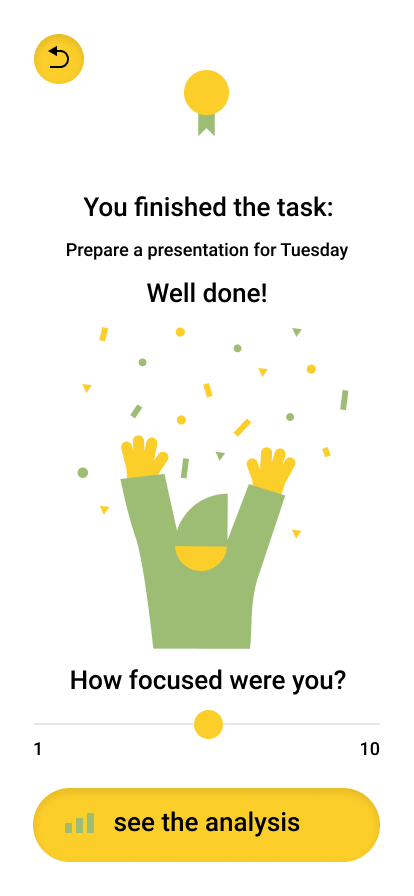
\includegraphics[width=0.8\linewidth]{images/sage_finish.png}
            \caption{Completing a task}
            \label{fig:old_sage_finish}
        \end{subfigure}%
        \begin{subfigure}{.3\textwidth}
            \centering
            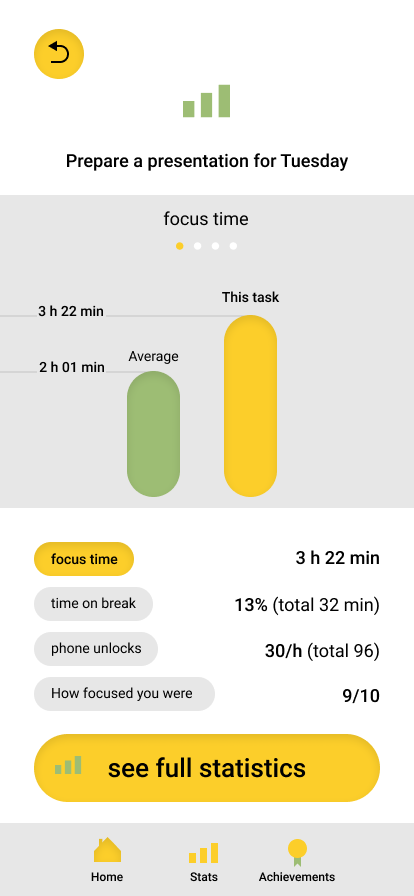
\includegraphics[width=0.8\linewidth]{images/sage_statistics.png}
            \caption{Usage statistics}
            \label{fig:old_sage_stats}
        \end{subfigure}%
        \caption{A few screens from the existing Sage app.}
        \label{fig:old_sage_achievements}
    \end{center}
\end{figure}

After granting the app permissions for notification access in an onboarding sequence, the app starts up and offers its core functionality: a task list. Users may create and edit tasks. Each task may be recurring daily, and may optionally block notifications. Users may then at any time start working on a task, triggering a running timer which may block all incoming notifications while active. A task can be completed, or returned to any time later with a break. All this activity is stored within the client and can be displayed to the user through graphs as a form of feedback on their productivity.

\subsection{Limiting issues}
While the legacy app passes as a starting effort, the concepts explored so far reveal many potential points for improvement. This naturally may have been the result of there only being a single developer at work. This is likely to occur again with this run of the project, and so this section serves as a potential guide for future work in identifying deficiencies in the app's user experience and building upon them. That said, there are several issues and limiting features with the current implementation of Sage, from both a UX design and software engineering perspective which we wish to prioritise in this run of the project:

\underline{Design \& User Experience}
\begin{itemize}
    \item The selected colour palette is dull, with no possible customisation on behalf of the user. Furthermore, colour contrast and shadows are not employed to draw attention to interactive elements within the app, reducing the enjoyability of the experience.
    \item All the assets and images are static, with no animation or movement to create the aforementioned dense and enjoyable app experience.
    \item Sizing of interactive elements is not well-standardised, and in most cases are oversized.
    \item Interface interactions are often not animated, which is not only potentially very jarring for the user, but also may result in a well-known concept known as change blindness \cite{simons1997change,simons2005change}, in which a user does not notice that an element of the interface has indeed changed. This directly translates to a higher amount of cognitive effort expenditure on the part of the user.
\end{itemize}

\underline{Software Engineering}
\begin{itemize}
    \item The notification blocking feature is faulty. The current implementation dismisses the notification using a callback function which is initiated when the notification is fired. This code is asynchronous to the actual firing of the notification, and therefore there exist edge cases in which it can fail.
    \item Currently implemented only as an Android app, with no extensibility to iOS, desktop or mobile web users. The features offered by native code APIs in Java and Kotlin are almost unused, and offer a lot of potential for attention-preserving features of the app.
    \item Completely local: no data backups or export, no online cloud synchronisation.
    \item No documented data model for the application, making continued development harder for newly-onboarded engineers.
\end{itemize}

\section{Concluding Remarks}
This chapter has explored the main concepts of neuroscience and user-experience design involved in app development. The existing app has been reviewed with a few starting points of critique, which is by no means exhaustive. The next step is to take these concepts back into a software engineering context and develop a set of requirements with an implementation plan for this run of the project.